\documentclass[12pt, letterpaper]{article}
\usepackage[utf8]{inputenc}
\usepackage{graphicx}
\usepackage{amsmath}
\usepackage{parskip}
\usepackage{tikz}
\usepackage{hyperref}

\newcommand{\externalLink}[2]{\emph{\underline{\href{#1}{#2}}}}


\title{Notes on Calculus III}
\author{Aaron Pierce}
\date{} % to remove date from \maketitle
\begin{document}

\maketitle

\tableofcontents

\newpage

\section{Early Chapters}

The beginning chapters aren't as noteworthy as the later ones, but they are still valuable. The following is a collection of the most important or interesting parts

\subsection{Dot Products}
Dot products are a form of vector multiplication. 

\textbf{Definition:} The dot product of two vectors ($\vec{A} \cdot \vec{B}$) is a real number given by the length of the projection of one vector onto another times the length of the vector being projected on.

That's a mouthful, and I like pictures.

\begin{figure}[h]
    \centering 
    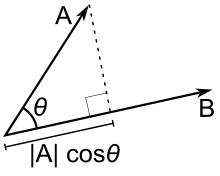
\includegraphics[width=0.30\textwidth]{dotproduct}
    \caption{A dot product in progress, as A is being projected onto B}
\end{figure}

Numerically, this projection is $|\vec{A}| cos(\theta) |\vec{B}|$, which corresponds to the length of the component of A that lies on B, times the length of B.

This definition derives some very useful other expressions, such as 

\begin{equation}
    \cos(\theta) = \frac{\vec{A} \cdot \vec{B}}{|\vec{A}||\vec{B}|}
\end{equation}
\begin{equation}
    comp_{\vec{B}} \vec{A} = \frac{\vec{A} \cdot \vec{B}}{|\vec{B}|} = \vec{A}\cos(\theta)
\end{equation}

Another way to define the dot product is the sum of the products of the components of the vectors. Another mouthful. The math is a easier to understand
\begin{gather*}
    \text{Let} \vec{A} = (A_1, A_2, ..., A_n)\\
    \text{Let} \vec{B} = (B_1, B_2, ..., B_n)\\
    \vec{A} \cdot \vec{B} = A_1 B_1 + A_2 B_2 + ... + A_n B_n
\end{gather*}
Let's call this the algebraic definition, as opposed to the projection or geometric definition from earlier.\\
This was surprising to me. How is this equivalent to the projection definition from earlier?
What helped me was realizing that this definition is equivalent to applying the geometric definition over the components of B.

\begin{gather*}
    \text{Let} \vec{A} = (A_1, A_2, A_3)\\
    \text{Let} \vec{B} = (B_1, B_2, B_3)\\
    \vec{B} = (B_1, 0, 0) + (0, B_2, 0) + (0, 0, B_3)\\
    \vec{A} \cdot \vec{B} =  \vec{A} \cdot (B_1, 0, 0) + \vec{A} \cdot (0, B_2, 0) + \vec{A} \cdot (0, 0, B_3)\\
    = A_1 B_1 + A_2 B_2 + A_3 B_3
\end{gather*}

This amounts to projecting A onto each component of B, which is just the corresponding component of A (projecting a vector onto a vertical vector is the same as taking the vertical component of the first vector and so on), 
multiplying their lengths, and adding all of those multiplications up, which gives us exactly the algebraic definition of the dot product


\subsection{Cross Products}
Cross products are, in my head, the counterpoint to a dot product. Whereas you can think of the dot product as what two vectors have in common (the component of one on another), the cross product gives the opposite, what the vectors do not have in common

Yet again we have two definitions, a geometric definition (again preferred by me), and an algebraic one

\textbf{Geometric Definition:} The cross product of two vectors ($\vec{A} \times \vec{B}$) is a new vector that is orthogonal to both vectors, whose length is equal to the area of the parallelogram formed by the two vectors being crossed.

\begin{figure}[h]
    \centering 
    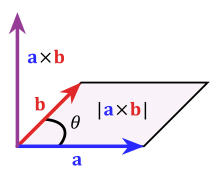
\includegraphics[width=0.30\textwidth]{crossproduct}
    \caption{The cross product}
\end{figure}

This seems a little strange. Why this definition of all things? It becomes a little clearer when we consider what the area of a parallelogram actually is.
This area is given by the base times the height, or for the vectors in the picture, $|\vec{A}| |\vec{B}|\sin(\theta)$, because $|\vec{A}|$ is the length of the base and $|\vec{B}|\sin(\theta)$ gives the height

So if the length of the cross product is this area, then $|\vec{A} \times \vec{B}| = |\vec{A}| |\vec{B}|\sin(\theta)$, and because we have introduced $\theta$, this becomes a very useful formula.

One use is to find the distance from a point and a line, which can be computed by crossing two vectors to form a parallelogram between the line and the point, and dividing by the length of its base to find the point's distance off the line.

It's worth specifically noting that the cross product returning an orthogonal vector is particularly powerful and useful. The length is arguably less useful of the two properties.

Actually computing this cross product is a little strange and unexplained to me, but I'll leave it here
\begin{align*}
    det
    \begin{vmatrix}
        \hat{i} & \hat{j} & \hat{k} \\
        A_1 & A_2 & A_3 \\
        B_1 & B_2 & B_3 \\
    \end{vmatrix}
\end{align*}

It's unclear to me why this produces an orthogonal vector, or why it is the length of the area of the parallelogram. Further research needed.

\subsection{Vector/Parametric Forms of Lines}

This is a short one. In $\mathbf{R}^2$, lines can be defined in point slope form. You start at a point, follow a slope, and you get your line. 
There's a similar concept in $\mathbf{R}^3$, with the vector form of a line. You start at a point, follow a vector, and you get your line.

The vector form of a line is as follows:
\begin{displaymath}
    L = \{\vec{r}(t) = P_0 + t\vec{d}\}
\end{displaymath}
Where $P_0$ is the point, and $\vec{d}$ is the direction vector of the line, the 3-space analog of a line's slope, and $t$ is some real number to scale the direction vector by.

This can also be rewritten in terms of each component of the vector that is returned by $\vec{r}(t)$, known as the parametric form of the line

\begin{gather*}
    x = P_{0x} + \vec{d}_xt\\
    y = P_{0y} + \vec{d}_yt\\
    z = P_{0z} + \vec{d}_zt\\
\end{gather*}


To compare to the other forms, all of the following draw the same line
\begin{gather*}
    y = x \\
    y - 0 = 1 (x - 0)\\
    L = \{\vec{r}(t) = (0, 0) + (1, 1)t\}\\
    \vec{r}(t)= (x, y): 
    \begin{cases}
        x = 0 + 1t\\
        y = 0 + 1t\\
    \end{cases}
\end{gather*}

As a sidenote, if you want to represent a line segement, instead of an infinite line, the idea is pretty cool. The line segement between two points starts at the first point and follows a vector formed by subtracting the points, and clamping $t$ between 0 and 1.

So the segment between $(a, b)$ and $(c, d)$ is represented by

\begin{gather*}
    \{\vec{r}(t) = (a,b) + t\left((c - a, d - b)\right)\}\\
    0 \leq t \leq 1
\end{gather*}

And checking this for $t = 1$ gives you 
\begin{displaymath}
    (a, b) + (c, d) - (a, b) = (c, d)
\end{displaymath}

And at 0 you get $(a, b)$, so the line will only exist between the two points. Pretty neat idea.

\subsection{Vector and 3D Functions}

Vector functions are pretty quick.
\begin{displaymath}
    \vec{v}(t) = (x(t), y(t), \dots)
\end{displaymath}

Their derivatives are the derivatives of the components of their vectors, and the usual derivative rules (product, quotient, etc.) work the way you would expect.

3D (or higher) functions are just as quick. Some function of x and y returns a z value, essentially taking the xy plane and raising it up along the z axis at each point $(x, y)$ to the value $f(x, y)$

If you want to take a derivative of these, you have to take some care, because there are now two axes in which you can move, so the notion of a derivative becomes a bit fuzzy. Enter the partial derivative

\textbf{Definition:} The partial derivative of a function is the derivative of a multidimensional function along a single axis. You take a slice of the surface created by the function, and the resulting single dimension of movement is the respect of the derivative. All other variables are treated as constants.

\begin{gather*}
    \frac{\partial}{\partial x}(f(x) = xy) = (1x^0)y \\
    \frac{\partial}{\partial y}(f(x) = xy) = x(1y^0)
\end{gather*}

\subsubsection{Tangent Planes and Linearization}
One of the uses of the derivative in 2 dimensions was to approximate a function. The tangent line is pretty close to the function at very small steps. In 3D, we need a tangent plane, to represent the two dimensions of movement we have.

To find a tangent line in $\textbf{R}^2$, we used a point and a slope $y - y_0 = f^\prime (x)(x-x_0)$. In $\textbf{R}^3$, we need two slopes, so 
\begin{displaymath}
    z - z_0 = \frac{\partial f}{\partial x}(x - x_0) + \frac{\partial f}{\partial y}(y - y_0)
\end{displaymath}
represents the tangent plane.

A little manipulation of that later and we get a way to linearize the function, which is pretty similar
\begin{displaymath}
    f(x, y) \approx f(a, b) + \frac{\partial f(a, b)}{\partial x}(x - a) + \frac{\partial f(a, b)}{\partial y}(y - b)
\end{displaymath}

Where $(a, b)$ is the point where you start, and $(x, y)$ is where you end up. Which amounts to starting at $(a, b)$, and walking a bit in the x multiplied by $\frac{\partial f}{\partial x}$, which is the slope (rise / run) in the x times the run, so you get the z that you should go up by, and you do the same in the y axis

We can think of tangent planes, tangent lines, and linearizations as applications of \textbf{differentials}. \textbf{Differentials} are generally linearizations of functions in whatever dimension the function is in. In two dimensions, the differential of a function is $dy = f^\prime (x)dx$, for any arbitrary dx. This gives you an equation for a tangent line. It's a slope times a change in the "run", so you get a rise.

In 3-space, the differential becomes slightly less clear because $f^\prime (x)$ now has to become partial derivatives. In 3-space $z$ changes instead of 2-space's $y$, but z can change in both the x and y axes. So to incorporate both of these, the total $dz$ will be dependent on $dz_x$ and $dz_y$.

We call then call $dz$ the total differential, defined by
\begin{gather*}
    dz = \frac{\partial f}{\partial x}(x, y)dx + \frac{\partial f}{\partial y}(x, y)dy  
\end{gather*}

This works out pretty well. When you bump x, what is the change in z. When you bump y, what is the change in z. The function that represents the total change in z is dependent on how much you bump x and y by. This then defines a tangent plane. You can bump x and y by any value, including zero, so this necessairly has to be a plane because it has to exist when either bump is zero, so it cannot be a line, because it must be able to move independently in two axes. It also doesn't make sense to be a line. How are you going to represent two dimensions of potential change in a one dimensional object.

\subsubsection{Quadratic Approximation}
While we're doing linear approximations, we may as well touch on quadratic approximation.

Quadratic approximation approximates a 3d function as a paraboloid instead of a line. This is pretty useful, as it's a good idea to approximate a 3D function with a 3D figure, instead of 1D lines.

This approximation is just an extension of a taylor polynomial. It looks like:
\begin{displaymath}
    Q_f(x) = f(x_0) + \nabla f(x_0)\cdot(x-x_0)+\frac{1}{2}(x-x_0)^T\mathbf{H}_f(x_0)(x-x_0)
\end{displaymath}
That looks pretty scary, let's break it down.

First off, $f(x_0)$ is the value of the function at the point $x_0$. This is the y-intercept, so to speak, of the approximation, or the point at which we want to start the paraboloid.

To that, we add $\nabla f(x_0)\cdot(x-x_0)$. This is a linear term. It's a vector of partial derivatives dotted with a vector of changes in position from the point $x_0$. This will build a tangent plane. We add the change in z with a nudge in x, and the change in z with a nudge in y, together, to get the total z change at any point away from $x_0$, which will be rendered as a plane.

Finally, we add the scary quadratic term. The first thing we should break down is $\mathbf{H}_f(x_0)(x-x_0)$. $\mathbf{H}_f$ is the Hessian matrix of f, a symmetric and square matrix of second order partial derivatives.
We evalute $\mathbf{H}_f(x_0)$ to be those partial derivatives at $x_0$. We then multiply this matrix by a column vector of the same changes we had earlier. In 3D this works out as follows:
\begin{gather*}
    \mathbf{H}_f(x_0) = \begin{bmatrix}
        \frac{\partial f}{\partial xx} & \frac{\partial f}{\partial xy}\\
        \frac{\partial f}{\partial yx} & \frac{\partial f}{\partial yy}\\
    \end{bmatrix}\\
    \mathbf{H}_f(x_0) \cdot (x - x_0) = \begin{bmatrix}
        \frac{\partial f}{\partial xx}(x_0) \cdot (x - x_0) + \frac{\partial f}{\partial xy}(x_0) \cdot (y-y_0)\\
        \frac{\partial f}{\partial yx}(x_0) \cdot (x - x_0) + \frac{\partial f}{\partial yy}(x_0) \cdot (y-y_0)\\ 
    \end{bmatrix}\\
    \frac{1}{2}(x-x_0)^T\mathbf{H}_f(x_0) \cdot (x - x_0) = 
    [x-x_0, y-y_0] \cdot \begin{bmatrix}
        \frac{\partial f}{\partial xx}(x_0) \cdot (x - x_0) + \frac{\partial f}{\partial xy}(x_0) \cdot (y-y_0)\\
        \frac{\partial f}{\partial yx}(x_0) \cdot (x - x_0) + \frac{\partial f}{\partial yy}(x_0) \cdot (y-y_0)\\ 
    \end{bmatrix}\\
    = \frac{1}{2}\frac{\partial f}{\partial xx}(x_0) \cdot (x-x_0)^2 + \frac{1}{2}\frac{\partial f}{\partial yy}(x_0) \cdot (y-y_0)^2 + \frac{\partial f}{\partial xy}(x_0) \cdot (x-x_0)(y-y_0)
\end{gather*}

So what's this look like then? We have taylor polynomials along x and y, which makes sense. The third term is (kind of) a taylor polynomial along some combination of the x and y directions.

This is sufficient for any direction between the axes. If you consider how this is being computed, it's whatever change in x, and whatever change in y, times the "slope" when you move along a partial derivative. They aren't independent, though, they're multiplied. If they were independent this would be another linear term. Because they are multiplied, this will create a parabolic term. (Consider when the x change is identical to the y change to see this, you end up squaring the change)

This is all super shallow though, and I need to spend more time on it. Further research needed.
\subsubsection{Contour Maps}
\label{sssec:Contour Maps}
Before we leave 3D functions it's worth mentioning contour maps because they're cool.\\
\begin{figure}[h]
    \centering 
    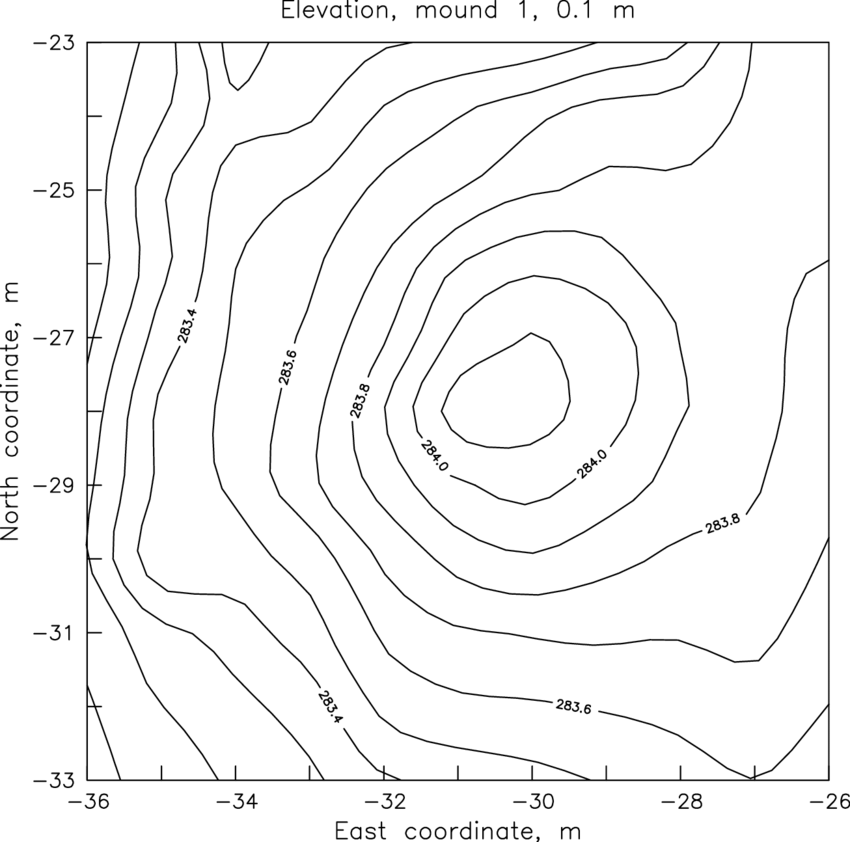
\includegraphics[width=0.5\textwidth]{contourmap}
    \caption{A contour map of some mound}
\end{figure}\\
The contour map of a 3D function is created by taking horizontal slices of the function at constant z values. This creates a neat way of visualizing these functions and will be useful for gradient fields later.

\newpage

\section{The Multidimensional Chain Rule}
What came before was all pretty clear the first time through. After this, though, was when the lectures started to get muddy, which inspired me to take some more detailed notes.

The multidimension chain rule is a weird one. I couldn't ever find a satisfactory answer, intuition, or explanation for why it made sense.

It helped to first consider the single dimension chain rule.

\begin{gather*}
    \text{For a function} f(g(x)), \text{Let} u = g(x) \\
    \frac{d}{dx} f(g(x)) = \frac{d}{dx} f(u) = f^\prime (u)\frac{du}{dx}\\
    \frac{du}{dx} = g^\prime (x)\\
    \frac{d}{dx} f(g(x)) = f^\prime (g(x)) g^\prime (x)
\end{gather*}

This is still pretty shallow for me. Seems more like a trick of notation than something that makes sense. If we go back and consider the derivative, though, it is definitionally the change in the value of the function when you change the input by a little bit.
\begin{gather*}
    f(x) = x^2\\
    f(x + dx) = (x+dx)^2\\
    = x^2 + 2xdx + {dx}^2\\
\end{gather*}

So when we nudge the function by $dx$, we get $x^2 + 2xdx + {dx}^2$. Before the nudge, the function was $x^2$, so the nudge changes the function by $2xdx + dx^2$. As $dx \to 0$, the value of $dx^2$ becomes very small and much less significant than $2xdx$. So when we nudge the function, its return value meaningfully changes by twice the value of the function at x, times the tiny nudge we made in the x, meaning that $f^\prime (x) = 2x\ dx$. This is where the power rule comes from.

When we nudge $f(g(x))$, we first nudge $g(x)$ by something, and the new value then becomes the input of $f$.

Let's ignore $g(x)$ for a second. So long as $g(x)$ is differentiable, then a small change in x would feel no different than if we nudged $g(x)$ as far as $f$ is concerned. 
Let's call $g(x)$ $u$ instead. A small nudge in $u$, du, corresponds to a change of $f^\prime (u)\ du$. The nudge du is itself the change in $g$ when you change x, that nudge is $g^\prime (x)\ dx$, which gives us the chain rule

\begin{gather*}
    \frac{d}{dx} f(g(x)) = f^\prime (u)\ du\\
    du = \frac{du}{dx}dx = g^\prime (x) dx\\
    \frac{d}{dx} f(g(x)) = f^\prime (g(x)) g^\prime (x)\ dx
\end{gather*}

Okay, so with the single dimensional chain rule out of the way we still have a beast left. Let's look at something easy first.
\begin{gather*}
    \text{Let} f(a, b) = a + b\\
    \text{What is } \frac{\partial}{\partial x}f(x^2, y^3).
\end{gather*}

The first thing to note is that a and b are private variables. The user who is feeding x's and y's into f has only indirect control over a and b. This means that taking a partial derivative with respect to a or b means nothing here, because the user inputting variables only knows what x and y are, and has never heard of a and b

Now, if you're just looking at this, you can just plug the functions in.

\begin{gather*}
    f(x^2, y^3) = x^2 + y^3\\
    \frac{\partial f}{\partial x} = 2x \\
    \frac{\partial f}{\partial y} = 3y^2
\end{gather*}

So you dont actually \emph{need} the chain rule. You could plug all of the functions in and take a partial derivative as normal.
However, if your functions get complex, say $f(u, v) = u^2sin^2(v)$ and $u$ and $v$ are themselves complicated, the partial derivatives get annoying really fast, so having a way to pre-compute this with a formula would be nice.

Let's take that example. for $f(sin(x), cos(y))$ what happens when we nudge x? Let's again call sin(x) u.

\begin{gather*}
    f(u, \cos(y)) = u^2\sin^2(\cos(y))\\
    \frac{\partial f}{\partial u} = 2u(\sin^2(\cos(y))\ du\\
    du = \frac{du}{dx}dx = \cos(x) dx\\
    \frac{\partial f}{\partial u} = 2\sin(x)(\sin^2(\cos(y))\cos(x)\\
\end{gather*}

Okay, that's all fine and good I guess, but what does it actually mean? The first thing we did was ignore sin(x). We want a change in f with a change in x, but a change in x makes a change in u, so we considered the change in u first.
The change caused by u was $\frac{\partial f}{\partial u}$, which is some term times du. So what is du? We really want a change with respect to x, so how can we find du in terms of dx?
We can take $\frac{du}{dx}$, because u depends on the variable x, and then multiply that by dx, so that we're left with du.

So if $\frac{\partial f}{\partial u}$ is something times du, and du is $\frac{du}{dx} dx$, then $\frac{\partial f}{\partial x} = \frac{\partial f}{\partial u} \frac{du}{dx}$
This makes some sense. If we nudge x and it doubles u, and if we nudge u and it doubles f, it makes sense that nudging x quadruples f (by multiplying, not squaring/exponentiating).

This is nice, but what if v also depends on x? Then we also have to think about v now! So when we nudge x it makes some change to u, which makes a change to f, but it also makes a change to v, which makes a change to f. What's the total change?
Well u and v aren't really related. The function can do whatever it wants with u and v, but no matter what, when you take a partial derivative of one, the other is constant. Unless they're the same thing, but that's beside the point.
Because they create two independent changes, you just add them. You change x, it changes u, which changes f. It also changes v, which changes f. u and v don't change each other, so you don't multiply them or compose them or do anything fancy. The partial derivative is just the sum of the changes.

This is all honestly shallow intuition. I still don't really get all of this. My saving grace is this tree
\begin{figure}[h]
    \centering 
    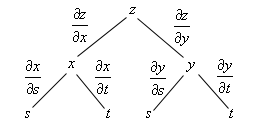
\includegraphics[width=0.5\textwidth]{chainruletree}
    \caption{How to compute a multidimensional chain rule}
\end{figure}

If you want \large$\frac{\partial z}{\partial s}$ \normalsize you follow all of the branches to s, multiply down the branch, and add the various branches. So,
\begin{gather*}
    \frac{\partial z}{\partial s} = \frac{\partial z}{\partial x} \frac{\partial x}{\partial s} + \frac{\partial z}{\partial y} \frac{\partial y}{\partial s}
\end{gather*}
This gives you what we had earlier. You keep unpacking various partial derivatives until you reach the variable you want, and then add all of the independent changes. I particularly like this tree becuase you could go 9 functions deep and it works the same way

My professor really likes emphasizing this derivative matrix $Df(x)$, which I think is supposed to be the \externalLink{https://en.wikipedia.org/wiki/Total_derivative}{Total Derivative} but everything about this seems like we'll get to it later so I'll skip it for now and instead focus on

\section{The Gradient and Directional Derivatives}
So first off, the gradient is, according to Grant Sanderson, weird. We'll start with the algebraic definition.

\begin{gather*}
    \nabla f(x, y, ...) = (\frac{\partial f}{\partial x}, \frac{\partial f}{\partial y}, \dots)
\end{gather*}

\begin{gather*}
    \text{Let} f(x, y) = x^2 sin(y)\\
    \frac{\partial f}{\partial x} = 2x\sin(y) \\
    \frac{\partial f}{\partial y} = x^2\cos(y) \\
    \nabla f(x, y) = (\frac{\partial f}{\partial x}, \frac{\partial f}{\partial y}) \\
    = (2x\sin(y), x^2\cos(y))
\end{gather*}

With this, it's important to note that the gradient is a \textbf{vector valued function}, which is a vector of all the partial derivatives of f. (Grant called this a full derivative, as it contains all of the partial derivatives).

A helpful way to think of this is
\begin{gather*}
    % \LARGE
    \nabla = \begin{bmatrix}
        \frac{\partial}{\partial x}\\
        \frac{\partial}{\partial y}\\
        \vdots
    \end{bmatrix}
    % \normalsize
\end{gather*}

And that $\nabla f(x)$ distributes $f(x)$ over that vector.

This is fine. It's a vector of partial derivatives, so what? What's neat about this is that it gives the direction of steepest ascent. That isn't at all intuitive at all, though. We just have a whole bunch of slopes in a whole bunch of directions. What gives?

First, a quick detour:

\subsection{Directional Derivatives}
What if instead of nudging a 3D function by x or y, we nudge it along some vector?
Pick some vector $\vec{v} = (a, b)$ to nudge along. This is like nudging by a in the x direction, and b in the y direction.
The directional derivative is
\begin{gather*}
    {\nabla}_{\vec{v}} f(x, y) 
    = a\frac{\partial f}{\partial x} + b\frac{\partial f}{\partial y} 
    = \vec{v} \cdot \nabla f(x, y)
\end{gather*}

Note the subscript of $\nabla$. Without it it's the gradient, as on the right, and with it it's the directional derivative.
Similar to a partial derivative, this corresponds to a slice of the graph of a 3D function from some plane that isn't necessarily parallel to either axis x or y.
That slice gives us some 2D function, where some step along that vector corresponds to a change in z, and some people write the directional vector as \Large $\frac{\partial f}{\partial \vec{v}}$ \normalsize to denote this.

That said, the line to remember is that the directional derivative is a partial derivative along some vector, instead of an axis. This is also results in giving you the slope of a graph when you walk along some vector, but you should be careful that when you are looking for the slope, you take a unit vector as the direction, otherwise you could get some multiple of the actual slope. 

Okay, with that in mind let's think about...

\subsection{Why the Gradient Gives the Direction of Steepest Ascent}

Imagine you are at a point on a 3D graph. In order to climb the graph as fast as possible, you want to find the largest slope from a directional derivative along some unit vector evaluated at your point. (A unit vector because $\vec{\infty}$ would always be the best choice)

To find this best vector, consider what the directional derivative actually is.

\begin{displaymath}
    \nabla_{\vec{v}} f(a, b) = \nabla f(a, b) \cdot \vec{v}
\end{displaymath}

If we want to maximize $\nabla_{\vec{v}} f(a, b)$, we really need to figure out what $\vec{v}$ dotted with $\nabla f(a, b)$ will give us the biggest slope (remember that $\vec{v}$ is a unit vector).

A dot product equals $|a| |b| \cos(\theta)$. When the vectors lie on the same line, ($\cos(\theta) = 1$) we get a maximal dot product, assuming $|a|\ \&\ |b|$ are fixed, which they are in a directional derivative.

Therefore, the best unit $\vec{v}$ will be on the same line as $\nabla f(a, b)$. It needs to be a unit vector, so take $\frac{\nabla f(a, b)}{|\nabla f(a, b)|}$ and you get a unit vector that returns the highest possible slope from a directional derivative

The gradient itself, evaluated at $(a, b)$, normalized, will then be the vector that, when traveled along, results in the greatest increase in altitude, because it is the highest slope, as we got from maximizing the directional derivative. Some more intuition is in the section on vector fields.

Pretty cool stuff. It's the backbone of the Gradient Descent Algorithm and I implemented it for a \externalLink{https://github.com/SAXTEN2011/LinearRegression/blob/master/index.js}{Linear Regression Model}

\subsection{Vector Fields}

Vector fields are pretty much what they sound like. It's a 2D plane of vectors, i.e. a function $f(x, y)$ that maps each point to some $\vec{v}$, which generalizes to some n-dimensional function mapping to some n-tuple

The construction of one such vector field can be done using the gradient operator. Taking $\nabla f(x, y)$ gives you some vector at the point $(x, y)$, and if you find the vector at every $(x, y)$ you get a vector field that we call the gradient field, because it was generated by the gradient operator. 

A neat thing to note is that the gradient field points in the direction of steepest ascent, because it is formed by the gradient. This is necessarily orthogonal to contour lines, as the steepest ascent is also the shortest path from one contour line to the next. If you zoom in super close on two nearby contour lines, they will eventually look like parallel lines. The shortest distance between parallel lines is an orthogonal path, so a gradient field will produce vectors orthogonal to a function's contour map.

\begin{figure}[h]
    \centering 
    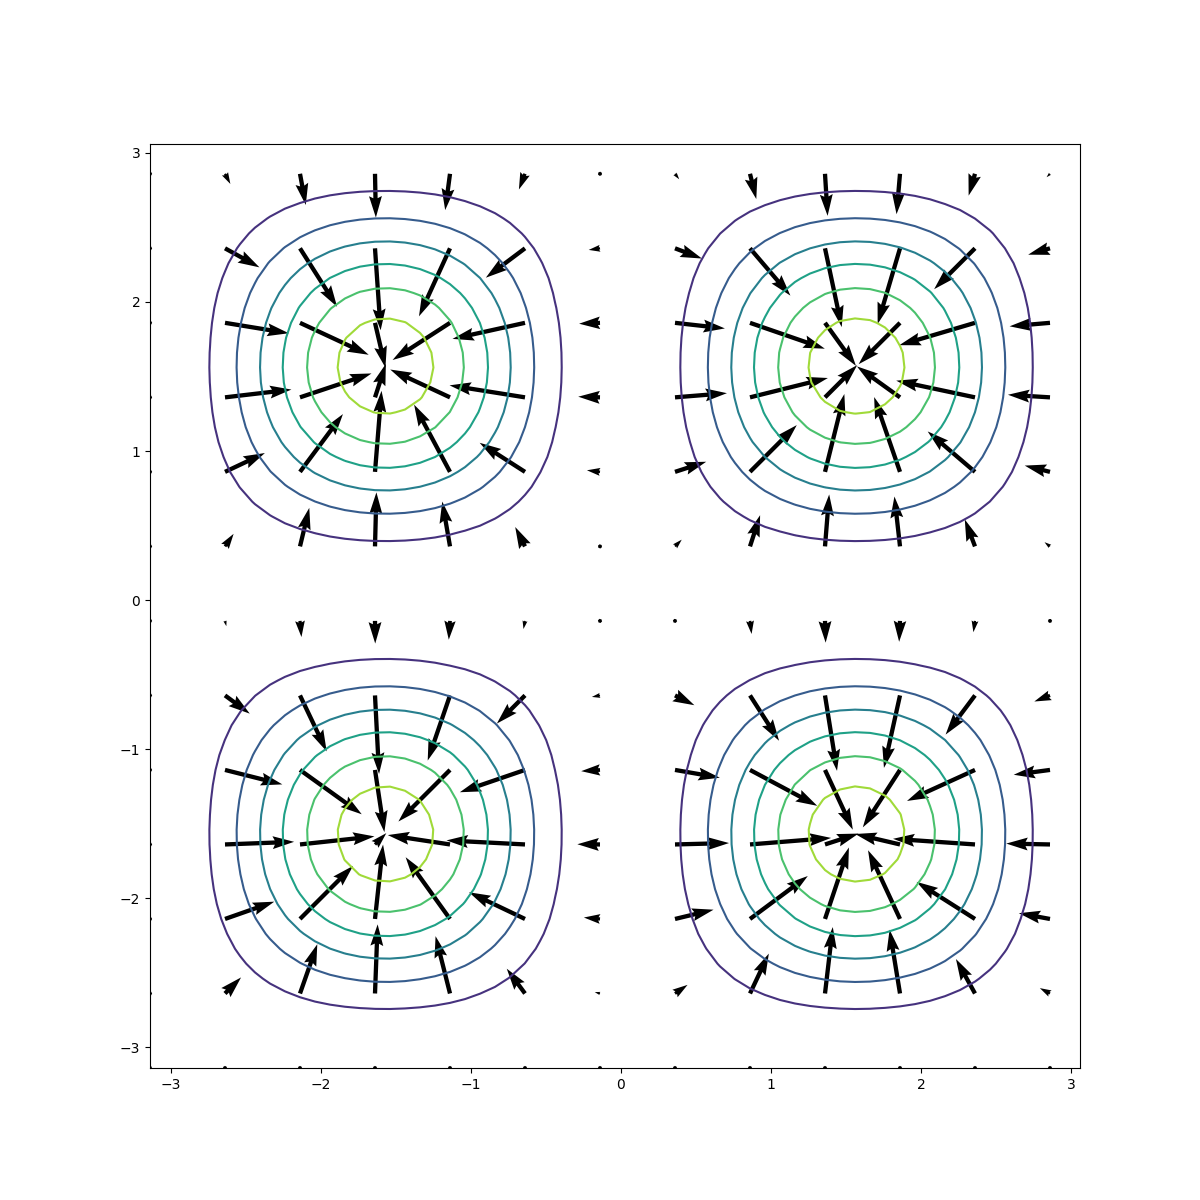
\includegraphics[width=0.75\textwidth]{orthogonalContour}
    \caption{A gradient field of $z = \sin(x)\sin(y)$ against its contour field. The vectors all point towards the peaks, which means orthogonal to the contours! Also, if they were parallel to the contours, you find a way to not ascend at all!}
\end{figure}

Okay so what. I get that being able to visualize a gradient field helps give some intuition for what following a gradient would mean, but why would I ever really need this outside of that intuition? 
The answer is on \externalLink{https://en.wikipedia.org/wiki/Vector_field\#Operations_on_vector_fields}{this wikipedia page} and I hope I take some notes on this. 
Further research needed.


\subsection{Tangent Planes to Level Surfaces}
If we want to find a tangent plane to a 3D surface, say $x^2 + y^2 + z^2 = 3$, we need to find some normal vector to the surface that we can make a plane from. To find this normal vector, we will be a little sneaky. We can think of this 3D function a level surface of a 4D function. A level surface is a slice in one axis of a function, so a level surface of a function, say $z = x^2 + y^2$, is just where $x^2 + y^2$ equals some constant $c$, i.e everywhere on the function that has a $z$ value equal to $c$, also known as a \hyperref[sssec:Contour Maps]{contour} of the function.

So we know that the gradient of a function points orthogonal to a contour line, because that is the fastest direction to the next contour line. Remember that the contour of a 3D function is some 2D curve, so the contour of a 4D curve is some 3D surface, and the gradient of a 4D function will result in a vector that is orthogonal to the 3D contour of the function. 

We can exploit this by thinking of some 3D surface as actually being some contour of a 4D function. So maybe we have some function $w = x^2 + y^2 + z^2$, in the 4D space defined by the axes x, y, z, and w. If we set $w$ to $3$, i.e take a level surface at $w=3$, then we get the sphere we led this section off with.

So to find a tangent plane to $x^2 + y^2 + z^2 = 3$, we should consider $x^2 + y^2 + z^2 = w$, a function of one higher dimension, and take a gradient. This will give a 3 vector that is necessarily orthogonal to the sphere because a 4D gradient will be orthogonal to its 3D contour. We can then use this gradient vector as the equation of a tangent plane $\vec{n}(p - p_0) = 0$, to find a tangent plane.

\section{Optimization}

In order to optimize a function, we look for maxima and minima in the function. 

In 2 dimensions this process is rather simple. You first find everywhere that the derivative is zero or undefined, so as to find points on the function where any change corresponds to increasing (or decreasing, so long as it happens in both directions) the value of the function at the point. You then check the second derivative of the function to see if the function is concave up (corresponding to a minima) or concave down (corresponding to a maxima).

In more than 2 dimensions we have the same general process. First we find where all partial derivatives are zero ($\nabla F(x, y) = \vec{0}$). If any of these partial derivatives weren't zero, then there would be a direction you could nudge the function in to increase or decrease the value of the function, thus your point is not an extrema. Put another way, the gradient points in the direction of steepest ascent, so if the gradient at a point is zero there is no direction that ascends, so you are at an extrema.
It was surprising to me that the gradient being zero was sufficient. It seemed reasonable that your derivative in the X and Y could be zero but between those axes it wouldn't be. This is wrong though. If you take a directional derivative you dot the direction vector with the gradient. So if the gradient is zero, so are all of the directional derivatives. 
(Putting it this way sounds like it would only work at maxima. To see why it works at minima, consider how you calculate the gradient. If you are at a minima the partial derivatives must be zero, because tangent lines are horizontal. A shallower way to consider this is to realize that any direction will correspond to steepest ascent at a minima, so the gradient either doesn't choose, or chooses all of them, which results in no change, whichever seems more reasonable to you.) 

Once we find all of the critical points, we need to decide if these points are maxima, minima, or saddle points. To find this, we need a second derivative test.

To find the second derivative of a multidimensional function, let's find the derivative of the gradient. Each term will need to be derived with respect to every other element, so the gradient becomes a matrix,
\begin{align*}
    \nabla f &= \begin{bmatrix}
        \frac{\partial f}{\partial x}\\
        \frac{\partial f}{\partial y}
    \end{bmatrix}
    \xrightarrow{Becomes}
    D f = \begin{bmatrix}
        \frac{\partial f}{\partial xx} & \frac{\partial f}{\partial xy}\\
        \frac{\partial f}{\partial yx} & \frac{\partial f}{\partial yy}\\  
    \end{bmatrix}
\end{align*}

This matrix is called a Hessian Matrix, a symmetric matrix of the second order partial derivatives of a function. This is the equivalent of a second derivative of a multivariable function, and we can use it for a sense of concavity.

First, if this is a saddle point, that means that two directions "disagree" in concavity. If either of $\frac{\partial f}{\partial x}$ or $\frac{\partial f}{\partial y}$ are zero, there's a saddle point. If they're both the same sign, they "agree" in concavity, and could well be a max or a min.
To encode this "agreement" we can multiply xx and yy second partial derivatives. If this number is positive, then both numbers were either positive or negative, so they agree. If the product is negative, one is positive and one is negative, and if the product is zero, then one of the directions was zero, and you have a saddle point.

If a critical point in 3D is a max or a min, the max/min will look like a paraboloid. If we find a taylor approximation of the 3D surface at a critical point, and the approximation looks like a paraboloid, then we know if it is indeed a max or a min, and its sign will distinguish between them.

We aren't really intersted in a very accurate approximation, we really just want to try to fit a paraboloid to it and hope that it works. Here's how we do this.

Firstly, we can linearly approximate the function. At any given point, the derivative with respect to some axis times the change in that axis, will give a tangent line. In 3D we want a tangent plane, we dot the gradient with a vector formed by $(x, y, z) - p_0$, where $p_0$ is the point at which you are taking the derivative and $(x, y, z)$ represents some new position along each axis

This information is encoded in the first derivative, but this only gives us where the function increases and decreases. At a critical point, this is zero, because they necessarily have horizontal tangent planes.

So we look next at the concavity of the function, encoded by the second derivative. When you bump x, it changes the function's rate of change in the x. If you multiply that rate of change by the change again, you get the change in z with respect to that bump in x. So the second derivative times the change (which is now a first derivative so to speak) times the change again (which is now a change in the function's value) will result in a quadratic approximation. You square the change to get some increase. To represent this, we hit the hessian matrix on both sides with the change vector. We've done lots of talking; here are some nice conscise symbols.

\begin{gather*}
    \text{Let } a = (x_0, y_0)\\
    f(x, y) \approx f(p_0) + \nabla f(p_0)(a - p_0) + (a - p_0) \cdot \mathbf{H_f}(p_0)(a - p_0)
\end{gather*}

But we only want to take this approximation at critical points, so $\nabla f$ is zero, and the linear term goes away!

So now our approximation is simply $f(p_0) + (a - p_0) \cdot \mathbf{H_f}(p_0)(a - p_0)$

$f(p_0)$ is the height of the function at our critical point. If the second term is always positive, then we only add height when we move away from the point, so the critical point is a min, and if its a max then the second term must always be negative.

So now we can determine whether the function is a max/min by just looking at the sign of $(a - p_0) \cdot \mathbf{H_f}(p_0)(a - p_0)$, which is very nice!

\end{document}